\documentclass{article}

\usepackage{fontspec}
\setmainfont{Open Sans-Regular}
\usepackage{tikz}
\usetikzlibrary{shapes.gates.logic.US}
\input{dft-tikz}
\definecolor{normalfillcolor}{gray}{0.7}
\setlength\paperwidth{30cm}
\setlength\paperheight{50cm}
\setlength\textheight{40cm}
\setlength\hoffset{-1in}
\newdimen\zigzagvert
\zigzagvert=5mm % Connections first go this far down, then zig-zag to
                % their target.
\pagestyle{empty}

\begin{document}
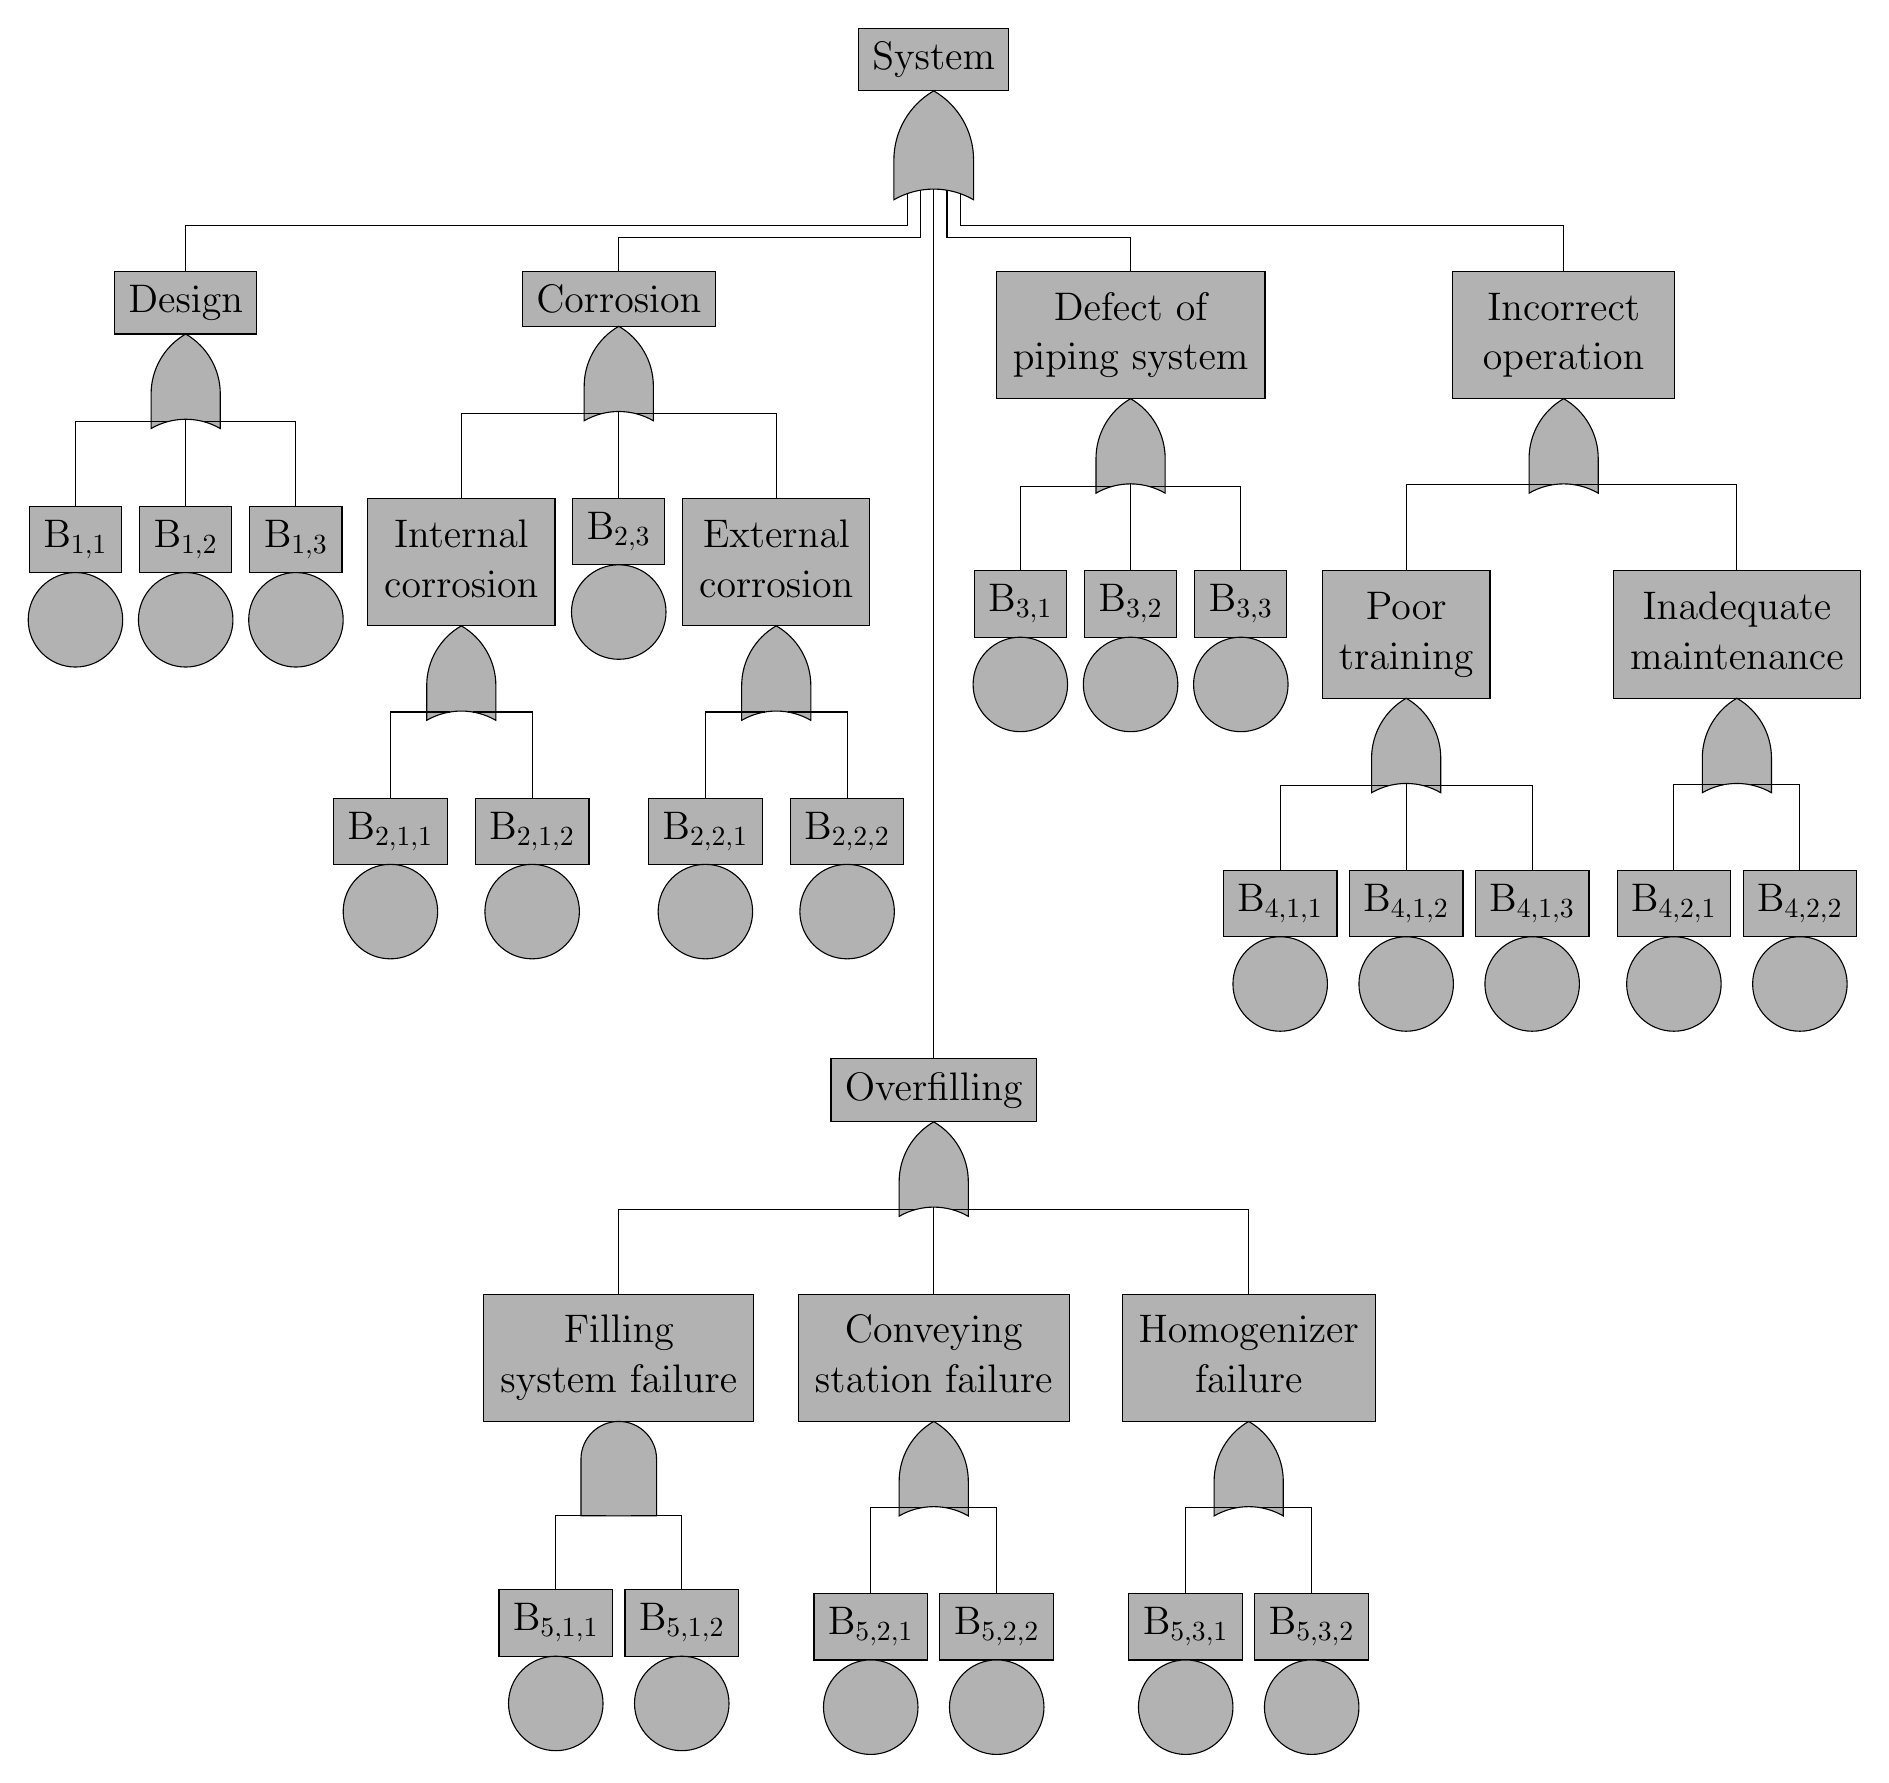
\begin{tikzpicture}[
	rectangle/.style={fill=normalfillcolor, inner sep=5pt},
	node distance=15mm,
	every node/.style={outer sep=0pt,font=\Large},
]
% Input 1 ignored (would be input count).
\def\basicevent#1[#2](#3)#4{
        \node[rectangle, draw, #2, minimum height=5.5mm, anchor=north](#3box){#4};
        \node[circle, minimum width=12mm, fill=normalfillcolor, draw,
		anchor=north] at (#3box.south) (#3) {};
}
% Input 1: Text in triangle.
\def\transferevent#1[#2](#3)#4{
        \node[rectangle, draw, #2, minimum height=5.5mm](#3box){#4};
	\path[draw, fill=normalfillcolor] (#3box.south)
		-- ++(-8mm, -15mm) -- ++(16mm, 0) -- (#3box.south);
	\path (#3box.south) ++ (0, -15mm) node[anchor=south] (#3) {#1};
}
\def\seqevent#1[#2](#3)#4{
        \node[rectangle, draw, #2, minimum height=1cm, minimum width=15mm](#3){};
	\node[anchor=north] at (#3.north) (#3box) {#4};
	\draw[->, line width=1mm] (#3.west) -- (#3.east);
}
\def\orevent#1[#2](#3)#4{
        \node[rectangle, draw, #2, minimum height=5.5mm, anchor=north](#3box){#4};
        \node[or gate US, minimum width=12mm, logic gate inputs=#1, rotate=90, fill=normalfillcolor, draw, anchor=output] at (#3box.south) (#3) {};
}
\def\andevent#1[#2](#3)#4{
        \node[rectangle, draw, #2, minimum height=5.5mm, anchor=north](#3box){#4};
        \node[and gate US, minimum width=12mm, logic gate inputs=#1, rotate=90, fill=normalfillcolor, draw, anchor=output] at (#3box.south) (#3) {};
}
% Input 1: Blank for normal, M for mirrored.
\def\sparegate#1[#2](#3)#4{
        \node[spare#1, fill=normalfillcolor, draw, anchor=north, #2]
		(#3) {};
	\node[anchor=north] at (#3.north) (#3box) {#4};
}
% Input 1 ignored (for consistency).
\def\fdepgate#1[#2](#3)#4{
        \node[fdep, fill=normalfillcolor, draw, anchor=north, #2]
		(#3) {};
	\node[anchor=north] at (#3.north) (#3box) {#4};
}
% \connectZZ{G.input}{vert. distance}{child}.
% Draw a line from G.input down by 'vert. distance', then zig-zag to
% child.
\def\connectcust#1#2#3{
	\draw[-] (#1) -- ++(0,#2) -| (#3box);
}
% \connect{G.input}{child} (Note: Only for vertical connections).
\def\connect#1#2{
	\connectcust{#1}{-\zigzagvert}{#2};
}
	\orevent{nnnnn}[](top){System}
	\orevent{nnn}[below of=top, xshift=-95mm](D){Design}
	\orevent{nnn}[below of=top, xshift=-40mm](C){Corrosion}
	\orevent{nnn}[below of=top, xshift=25mm](P)
		{\hspace*{-5pt}\begin{tabular}{c}Defect of\\piping
		system\end{tabular}\hspace*{-5pt}}
	\orevent{nnn}[below of=top, yshift=-10cm](OF){Overfilling}
	\orevent{nn}[below of=top, xshift=8cm](IO)
		{\begin{tabular}{c}Incorrect\\operation\end{tabular}}
	\connectcust{top.input 1}{-4mm}{D}
	\connectcust{top.input 2}{-6mm}{C}
	\connectcust{top.input 3}{-8mm}{OF}
	\connectcust{top.input 4}{-6mm}{P}
	\connectcust{top.input 5}{-4mm}{IO}
	\basicevent [below of=D, xshift=-14mm](B11){B$_{1,1}$}
	\basicevent [below of=D](B12){B$_{1,2}$}
	\basicevent [below of=D, xshift=14mm](B13){B$_{1,3}$}
	\connect{D.input 1}{B11}
	\connect{D.input 2}{B12}
	\connect{D.input 3}{B13}

	\orevent{nn}[below of=C, xshift=-2cm](IC)
		{\hspace*{-5pt}\begin{tabular}{c}Internal\\corrosion\end{tabular}\hspace*{-5pt}}
	\orevent{nn}[below of=C, xshift=2cm](EC)
		{\hspace*{-5pt}\begin{tabular}{c}External\\corrosion\end{tabular}\hspace*{-5pt}}
	\basicevent [below of=C](B23){B$_{2,3}$}
	\connect{C.input 1}{IC}
	\connect{C.input 2}{B23}
	\connect{C.input 3}{EC}
	\basicevent [below of=IC, xshift=-9mm](B211){B$_{2,1,1}$}
	\basicevent [below of=IC, xshift=9mm](B212){B$_{2,1,2}$}
	\connect{IC.input 1}{B211}
	\connect{IC.input 2}{B212}
	\basicevent [below of=EC, xshift=-9mm](B221){B$_{2,2,1}$}
	\basicevent [below of=EC, xshift=9mm](B222){B$_{2,2,2}$}
	\connect{EC.input 1}{B221}
	\connect{EC.input 2}{B222}

	\basicevent [below of=P, xshift=-14mm](B31){B$_{3,1}$}
	\basicevent [below of=P](B32){B$_{3,2}$}
	\basicevent [below of=P, xshift=14mm](B33){B$_{3,3}$}
	\connect{P.input 1}{B31}
	\connect{P.input 2}{B32}
	\connect{P.input 3}{B33}

	\orevent{nnn}[below of=IO, xshift=-2cm](PT)
		{\hspace*{-5pt}\begin{tabular}{c}Poor\\training\end{tabular}\hspace*{-5pt}}
	\orevent{nn}[below of=IO, xshift=22mm](IM)
		{\hspace*{-5pt}\begin{tabular}{c}Inadequate\\maintenance\end{tabular}\hspace*{-5pt}}
	\connect{IO.input 1}{PT}
	\connect{IO.input 2}{IM}

	\basicevent [below of=PT, xshift=-16mm](B411){B$_{4,1,1}$}
	\basicevent [below of=PT](B412){B$_{4,1,2}$}
	\basicevent [below of=PT, xshift=16mm](B413){B$_{4,1,3}$}
	\connect{PT.input 1}{B411}
	\connect{PT.input 2}{B412}
	\connect{PT.input 3}{B413}
	\basicevent [below of=IM, xshift=-8mm](B421){B$_{4,2,1}$}
	\basicevent [below of=IM, xshift=8mm](B422){B$_{4,2,2}$}
	\connect{IM.input 1}{B421}
	\connect{IM.input 2}{B422}

	\andevent{nn}[below of=OF, xshift=-4cm](FS)
		{\hspace*{-5pt}\begin{tabular}{c}Filling\\system failure\end{tabular}\hspace*{-5pt}}
	\orevent{nn}[below of=OF](CS)
		{\hspace*{-5pt}\begin{tabular}{c}Conveying\\station failure\end{tabular}\hspace*{-5pt}}
	\orevent{nn}[below of=OF, xshift=4cm](H)
		{\hspace*{-5pt}\begin{tabular}{c}Homogenizer\\failure\end{tabular}\hspace*{-5pt}}
	\connect{OF.input 1}{FS}
	\connect{OF.input 2}{CS}
	\connect{OF.input 3}{H}

	\basicevent [below of=FS, xshift=-8mm](B511){B$_{5,1,1}$}
	\basicevent [below of=FS, xshift=8mm](B512){B$_{5,1,2}$}
	\connect{FS.input 1}{B511}
	\connect{FS.input 2}{B512}
	\basicevent [below of=CS, xshift=-8mm](B521){B$_{5,2,1}$}
	\basicevent [below of=CS, xshift=8mm](B522){B$_{5,2,2}$}
	\connect{CS.input 1}{B521}
	\connect{CS.input 2}{B522}
	\basicevent [below of=H, xshift=-8mm](B531){B$_{5,3,1}$}
	\basicevent [below of=H, xshift=8mm](B532){B$_{5,3,2}$}
	\connect{H.input 1}{B531}
	\connect{H.input 2}{B532}
\end{tikzpicture}
\end{document}
